\documentclass[10pt]{beamer}

\usetheme{metropolis}
\usepackage{appendixnumberbeamer}

\usepackage{booktabs}
\usepackage[scale=2]{ccicons}

\usepackage{pgfplots}
\usepgfplotslibrary{dateplot}

\usepackage{xspace}
\newcommand{\themename}{\textbf{\textsc{metropolis}}\xspace}

\usepackage{tikz}
\usepackage{tikz-3dplot}
\usetikzlibrary{decorations.markings}
\tikzset{isometricXYZ/.style={x={(-0.866cm,-0.5cm)}, y={(0.866cm,-0.5cm)}, z={(0cm,1cm)}}}

\usepackage[]{algorithm2e}

\title{Gesture Interface}
\subtitle{A Naive Framework}
\date{\today}
\author{Pan An (Andy)}
\institute{National University of Singapore}
% \titlegraphic{\hfill
\includegraphics[height=1.5cm]{logo.pdf}}

\begin{document}

\maketitle

\begin{frame}{Table of Contents}
  \setbeamertemplate{section in toc}[sections numbered]
  \tableofcontents[hideallsubsections]
\end{frame}

\section{Introduction}

\begin{frame}
  \frametitle{Overview}
  \begin{block}{Gestures}
    \begin{itemize}
    \item Spatial Motions
    \item Finger Motions
    \item Muscles and other Biosignals
    \item Possibility with hybrid hardwares
    \end{itemize}
  \end{block}

  \begin{block}{Tasks(What we can do with machines)}
    \begin{itemize}
    \item Motions and movements
    \item Objects and obstacles
    \item Complex tasks and command compressing
    \end{itemize}
  \end{block}
\end{frame}

\begin{frame}[fragile]{Gestures}
  \begin{columns}[T,onlytextwidth]
    \column{0.5\textwidth}
    \begin{figure}[!ht]
      \centering
      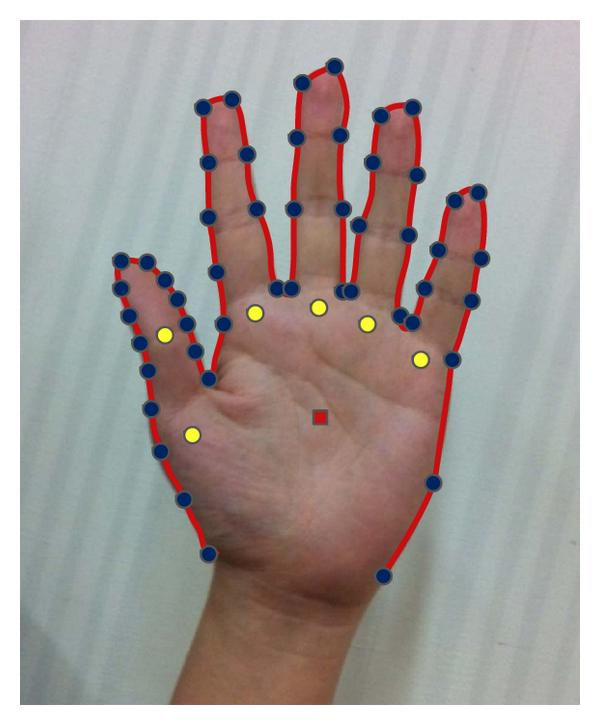
\includegraphics[width=3cm]{ges.jpg}
      \caption{\scriptsize{} Example of Hand Gesture.}
      \label{fig:gesture}
    \end{figure}
    \begin{block}{Color Based Method}
      \scriptsize
      The above picture is an example of color based gesture
      recognition. Color based algorithms are normally heavily relying
      on background color. 
    \end{block}
    \column{0.5\textwidth}

    
    \metroset{block=fill}
    \vspace{8mm}
    \begin{block}{Spatial Motions}
      Swipe, tracking, clapping...
    \end{block}

    \begin{block}{Finger Motions}
      Grabbing, rub, pointing and etc.
    \end{block}

    \begin{block}{Muscles and Other Biosignals}
      All Involves hardwares.
    \end{block}

    \begin{alertblock}{Note}
      Naive camera based gestures are used.  
    \end{alertblock}
  \end{columns}
\end{frame}



\section{Inverse Kinematics}

\begin{frame}
  \frametitle{IK Algorithms}
  \begin{itemize}
  \item Cyclic Coordinate Descent
  \item Jacobian Transpose
  \item FABRIK
  \item Neural Network
  \end{itemize}
\end{frame}

\begin{frame}
  \frametitle{Cyclic Coordinate Descent}
  \only<1>{
    \begin{columns}
      \column{0.5\textwidth}
      \begin{figure}[!ht]
        \centering
        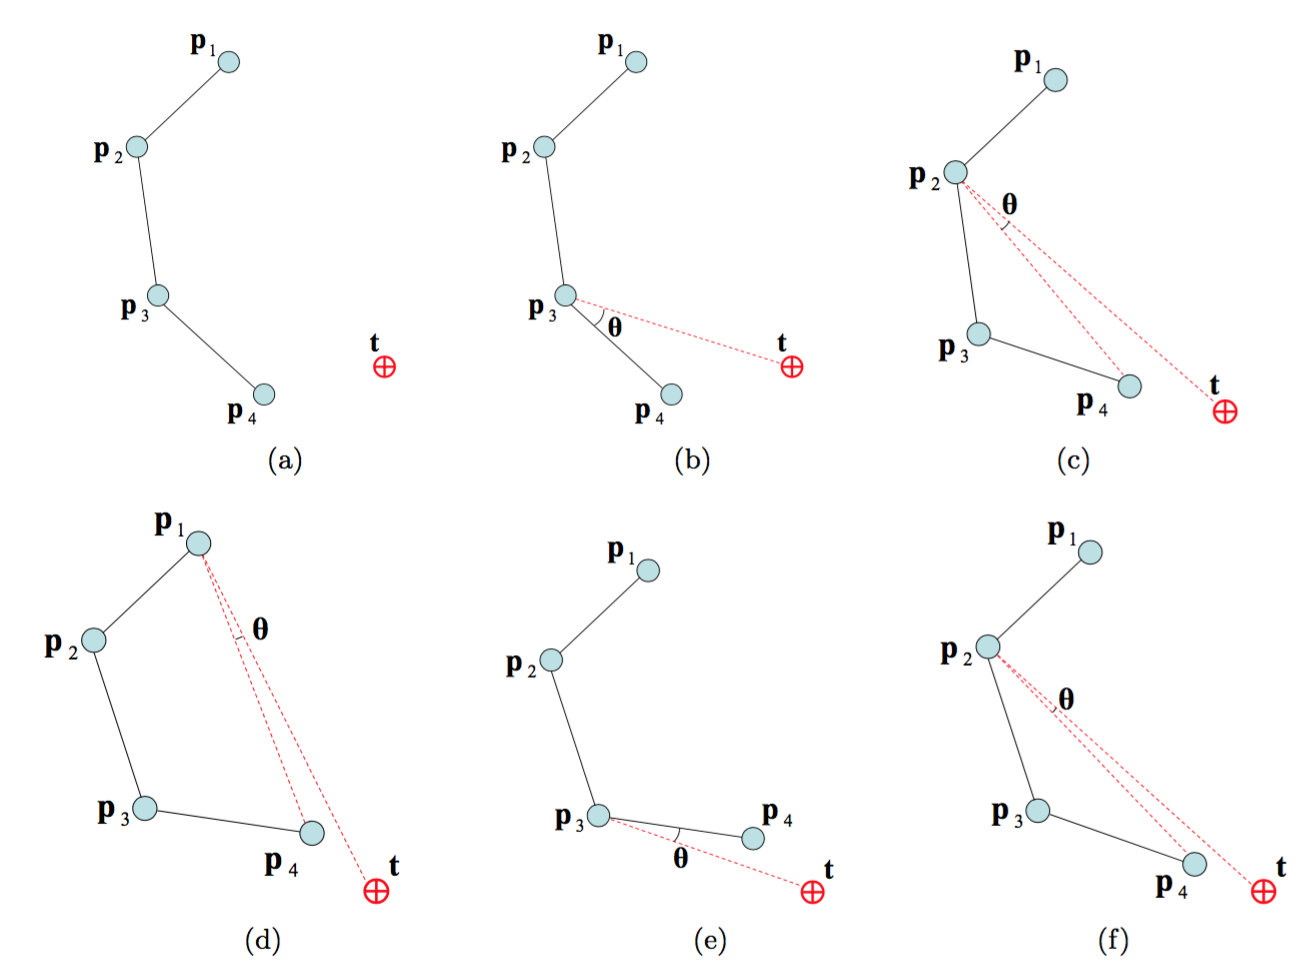
\includegraphics[width=5cm]{ccd.png}
      \end{figure}

      \column{0.5\textwidth}

      \metroset{block=fill}
      \vspace{6mm}
      \begin{block}{Basic Idea}
        \begin{itemize}
        \item Greedy
        \item Iterative
        \item Does not care whether the target is within range
        \end{itemize}
      \end{block}

      \begin{block}{Why}
        WangXin made the CCD work.
      \end{block}
    \end{columns}
  }
\end{frame}

\begin{frame}
  \frametitle{Jacobian Transpose}
  \begin{columns}
    \column{0.5\textwidth}
    \begin{figure}[!ht]
      \centering
      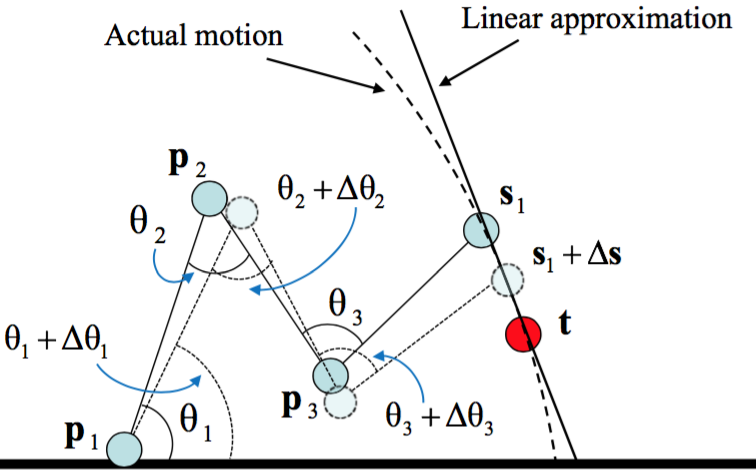
\includegraphics[width = 6cm]{jacob.png}
      \caption{Jacobian Transpose}
      \label{fig:jacob}
    \end{figure}

    \column{0.5\textwidth}

    \only<1>{

      \begin{block}{Definitions}
        \begin{itemize}
        \item[] $J$ ~ Partial Derivation of the entire chain system.
        \item[] $\pmb\theta$ ~ Vector of $\theta$ values.
        \item[] $\pmb s$ ~ Vector of end effectors.
        \item[] $\pmb p_j$ ~ Position of the joints.
        \end{itemize}
      \end{block}

      \metroset{block=fill}
      \begin{block}{Jacobian Matrix}
        $$J({\pmb\theta}_{ij})=(\frac{\partial{\pmb s}_i}{\partial\theta_{j}})_{ij}$$
      \end{block}

      Where $i = 1, ..., k$ and $j = 1, ..., n$. In this case $k = 1$
      and $n = 3$.
    }
    \only<2>{
      \metroset{block=fill}
      \begin{block}{Jacobian Transpose}
        Jacobian Transpose is to move the angles with a step of
        $$\Delta \theta = \alpha J^T \vec{\pmb e}$$

        Where $\pmb e$ is the vector of direction of the step and
        $\alpha$ is the selected step size.
      \end{block}
    }

  \end{columns}

\end{frame}



\begin{frame}
  \frametitle{FABRIK}
  \begin{columns}
    \column{0.5\textwidth}
    \begin{figure}[!ht]
      \centering
      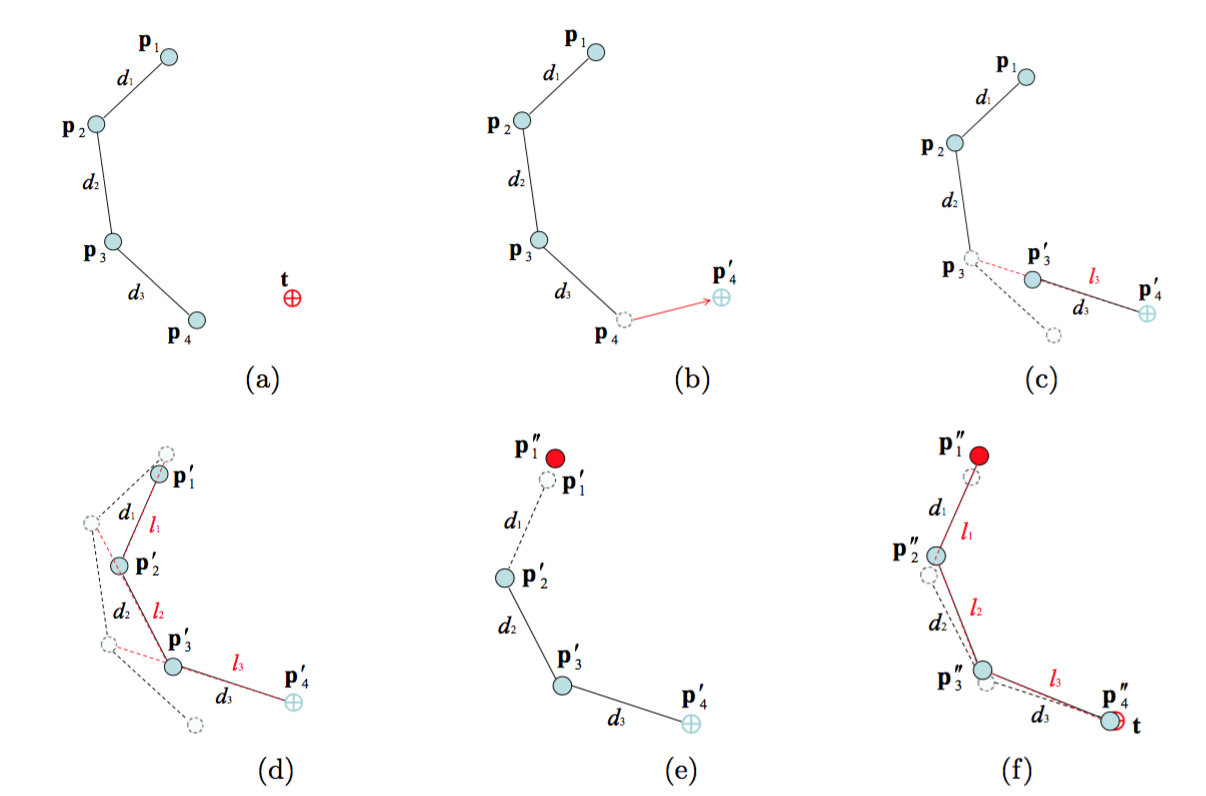
\includegraphics[width=6cm]{fab.png}
      \caption{FABRIK}
      \label{fig:fab}
    \end{figure}

    \column{0.5\textwidth}

    \only<1>{
      \begin{block}{FABRIK}
        Stands for Forward And Backward Reaching Inverse Kinematics.
      \end{block}

      \begin{block}{Definitions}
        \begin{itemize}
        \item[] $\pmb t$ ~ Vector of targets.
        \item[] $d_i$ ~ Distance between each joint $d_i = |\pmb p_{i+1}
          - \pmb p_i|$
        \end{itemize}
      \end{block}}
    \only<2>{
      \scriptsize
      \begin{algorithm}[H]
        \KwData{$\pmb d, \pmb t, \pmb p$}
        \KwResult{The new joint positions $\pmb p$}
        initialization\;
        \eIf{Target is not within range}{
          point directly to the target and return\;
        }{
          $\pmb b=\pmb p_1$ and $dif_A = |\pmb p_n-\pmb t|$\;
          \While{$dif_A>tolerance$}{
            $\pmb p_n=\pmb t$\;
            \For{$i = n-1,  ..., 1$}{
              $r_i = |\pmb p_{i+1}-\pmb p_i|$\;
              $\lambda_i = \frac{d_i}{r_i}$\;
              $\pmb p_i = (i-\lambda_i)\pmb p_{i+1} - \lambda_i \pmb p_i$\;
            }
            $\pmb p_1 = \pmb b$\;
            \For{$i = 1,  ..., n-1$}{
              $r_i = |\pmb p_{i+1}-\pmb p_i|$\;
              $\lambda_i = \frac{d_i}{r_i}$\;
              $\pmb p_i = (i-\lambda_i)\pmb p_{i+1} - \lambda_i \pmb p_i$\;
            }
          }
        }
      \end{algorithm}
    }
  \end{columns}

\end{frame}


\begin{frame}
  \frametitle{FABRIK Constraints}
  \begin{figure}[!ht]
    \centering
    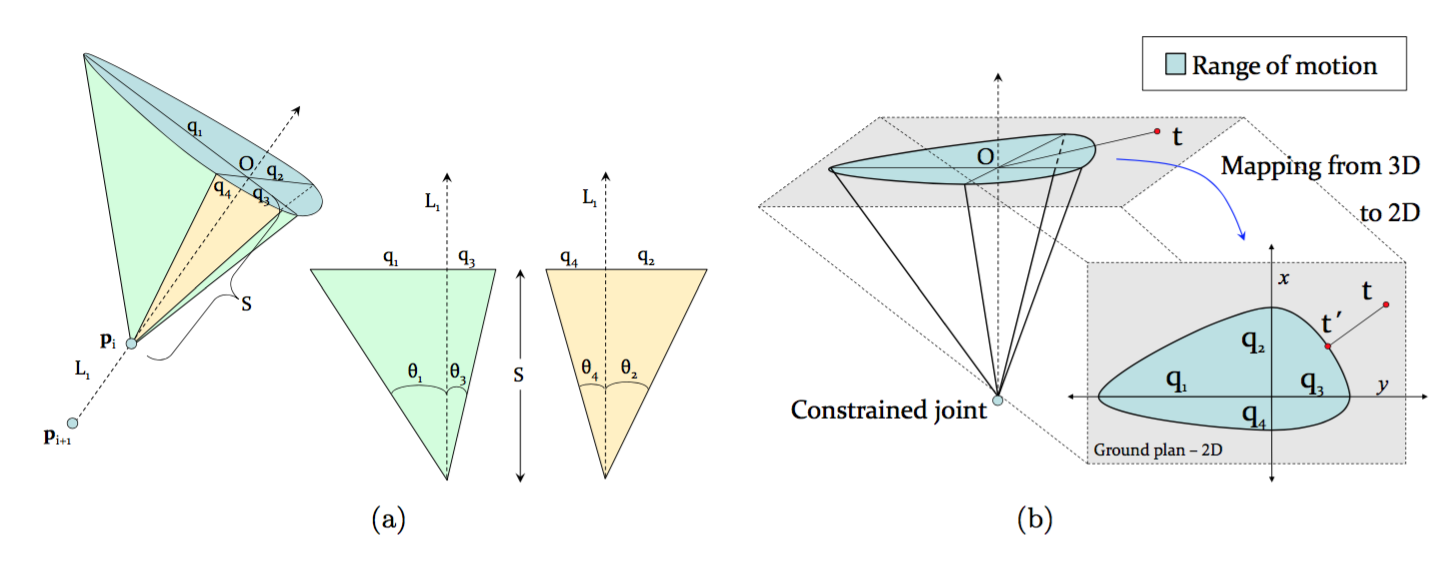
\includegraphics[width=10cm]{constraints.png}
    \caption{Example of Constraints in a Joint System}
    \label{fig:constraints}
  \end{figure}
\end{frame}

\begin{frame}[fragile]
  \frametitle{Reachable Space}
  \begin{figure}[!ht]\centering

    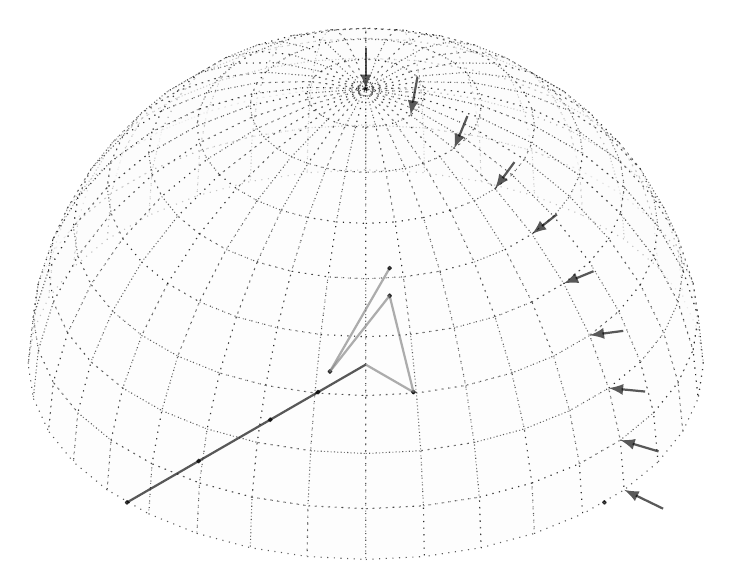
\begin{tikzpicture}[scale=3.5, isometricXYZ, line join=round,
      opacity=.65, text opacity=1.0,%
      >=latex,
      inner sep=0pt,%
      outer sep=2pt,%
      ]
      \def\h{5}

      \newcommand{\quadrant}[2]{
        \foreach \f in {85,75,...,5}
        \foreach \t in {#1}
        \draw [dotted, fill=#2]
        ({sin(\f - \h)*cos(\t - \h)}, {sin(\f - \h)*sin(\t - \h)}, {cos(\f - \h)})
        -- ({sin(\f - \h)*cos(\t + \h)}, {sin(\f - \h)*sin(\t + \h)}, {cos(\f - \h)})
        -- ({sin(\f + \h)*cos(\t + \h)}, {sin(\f + \h)*sin(\t + \h)}, {cos(\f + \h)})
        -- ({sin(\f + \h)*cos(\t - \h)}, {sin(\f + \h)*sin(\t - \h)}, {cos(\f + \h)})
        -- cycle;
      }

      % Quadrants
      \quadrant{130,140,...,310}{gray!2}
      \quadrant{-50,-40,...,130}{gray!2}


      \draw[thick] (0,0,0) -- (1,0,0) node[right] {};
      \draw[gray, thick] (0,0,0) -- (0,0.2,0) node[right] {};
      \draw plot [mark=*, mark size=0.2] coordinates{(0,0.2,0)};

      \draw[gray, thick] (0.2,0.3,0.5) -- (0,0.2,0) node[right] {};
      \draw plot [mark=*, mark size=0.2] coordinates{(0.2,0.3,0.5)};

      \draw[gray, thick] (0.2,0.3,0.5) -- (0.5,0.35,0.4) node[right] {};
      \draw plot [mark=*, mark size=0.2] coordinates{(0.5,0.35,0.4)};

      \draw[gray, thick] (0.1,0.2,0.5) -- (0.5,0.35,0.4) node[right] {};
      \draw plot [mark=*, mark size=0.2] coordinates{(0.1,0.2,0.5)};

      \draw plot [mark=*, mark size=0.2] coordinates{(0,1,0)};

      \draw plot [mark=*, mark size=0.2] coordinates{(0.2,0,0)};
      \draw plot [mark=*, mark size=0.2] coordinates{(0.4,0,0)};
      \draw plot [mark=*, mark size=0.2] coordinates{(0.7,0,0)};
      \draw plot [mark=*, mark size=0.2] coordinates{(1,0,0)};

      % View arrows
      \def\l{1.15}
      \foreach \f in {0,10,...,90}
      \foreach \t in {95}
      \draw [black, ->, thick]
      ({\l*sin(\f)*cos(\t)},{\l*sin(\f)*sin(\t)},{\l*cos(\f)})
      -- ({sin(\f)*cos(\t)},{sin(\f)*sin(\t)},{cos(\f)});

      % Circles in local coordinate system of the arrows
      % \foreach \f in {0,10,...,90}
      % \foreach \t in {95}
      % {
      % \def\PosX{{\l*sin(\f)*cos(\t)}}
      % \def\PosY{{\l*sin(\f)*sin(\t)}}
      % \def\PosZ{{\l*cos(\f)}}
      % \def\Pos{(\PosX, \PosY, \PosZ)}

      % \begin{scope}[rotate around={\f:\Pos}]
      %   \draw[->,red,thick] \Pos circle (0.07);
      % \end{scope}
      % };
    \end{tikzpicture}

    \caption{Reachable Space of a Fully Free Robot Arm}
    \label{fig:space}
  \end{figure}
\end{frame}

\begin{frame}
  \frametitle{Reachable Space for UR10}
  \pgfmathsetmacro\x{cos(105)*4}
  \pgfmathsetmacro\y{sin(105)*4}
  \begin{figure}[!ht]
    \centering
    \begin{tikzpicture}
      \draw[thick] (4,0) arc (0:75:4);
      \draw[thick] (\x,\y) arc (105:180:4);
      \draw[thick] (-4,0) -- (4,0);
      \draw[thick] (\x,\y) -- (-\x,\y);
      \draw[thick] (0,0) -- (0, 0.2);
      \draw[thick] (0,0.2) -- (-0.5,0.2);
      \draw[thick] (-0.5,0.2) -- (-0.5,1.6);
      \draw[thick] (-0.5,1.6) -- (0, 1.6);
      \draw[thick] (0, 1.6) -- (0,3.2);
      \draw[thick] (0, 3.2) -- (-0.3, 3.2);
      \draw[thick] (-0.3, \y) -- (-0.3, 3.2);
      \draw[line width = 0.5mm] (-0.3, \y) -- (\x, \y);
    \end{tikzpicture}
    
    \caption{Reachable Space for UR10}
    \label{fig:ur}
  \end{figure}
\end{frame}

%%% Local Variables:
%%% mode: latex
%%% TeX-master: "demo"
%%% End:



%%% Local Variables:
%%% mode: latex
%%% TeX-master: "demo"
%%% End:


\section{Learning Methods}
\begin{frame}
  \frametitle{Actions(Scenarios)}

  \begin{columns}
    \column{0.5\textwidth}
    \begin{figure}[!ht]
      \centering
      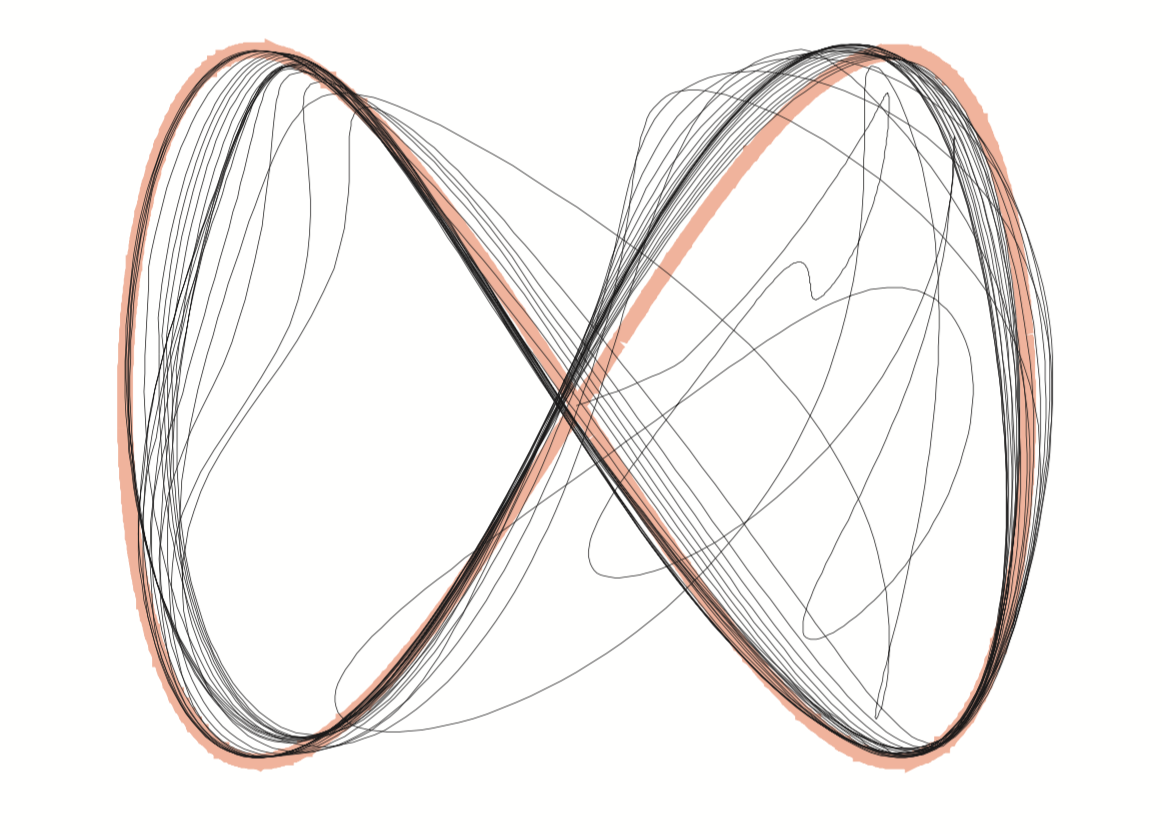
\includegraphics[width=6cm]{scene.png}
    \end{figure}

    \column{0.5\textwidth}
    \metroset{block=fill}
    \begin{block}{Natural Gesture of a Robot}
      \begin{itemize}
      \item[] Unpredictability
      \item[] Robustness
      \item[] Gesture when reaching the end effector
      \end{itemize}
    \end{block}

    \begin{block}{Learning Method}
      \begin{itemize}
      \item[] Monte Carlo(policy search)
      \item[] Dynamic Programming(value function)
      \item[] Neural Network
      \end{itemize}
    \end{block}


  \end{columns}
\end{frame}

\begin{frame}
  \frametitle{Model}
  \only<1>{
    \begin{figure}[!ht]
      \centering
      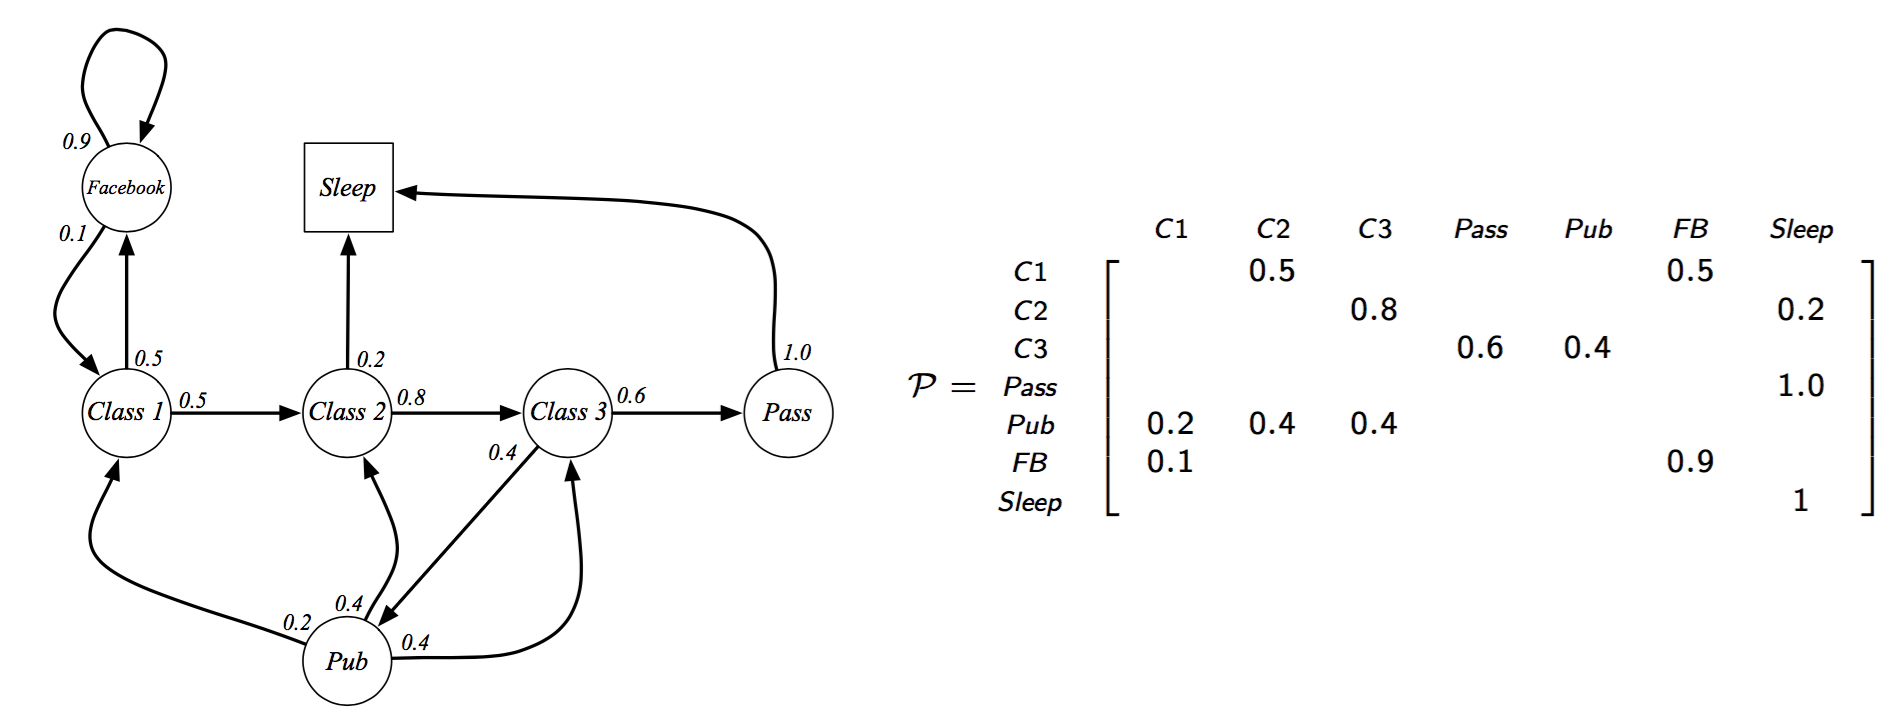
\includegraphics[width=11cm]{mdp.png}
    \end{figure}
  }
  \only<2>{
    \begin{block}{Definitions}
      \begin{itemize}
      \item[] $\pi$ ~ Policy: mapping from states to actions
      \item[] $S$ ~ A set of States
      \item[] $A$ ~ A set of Actions
      \item[] $R$ ~ Reward Function
      \item[] $P$ ~ State transition function
      \item[] $v(s)$ ~ State Value Function of a MRP
      \item[] $\gamma$ ~ Discount Function, $\gamma \in [0, 1]$
      \end{itemize}
    \end{block}
  }
  \only<3>{
    \begin{figure}[!ht]
      \centering
      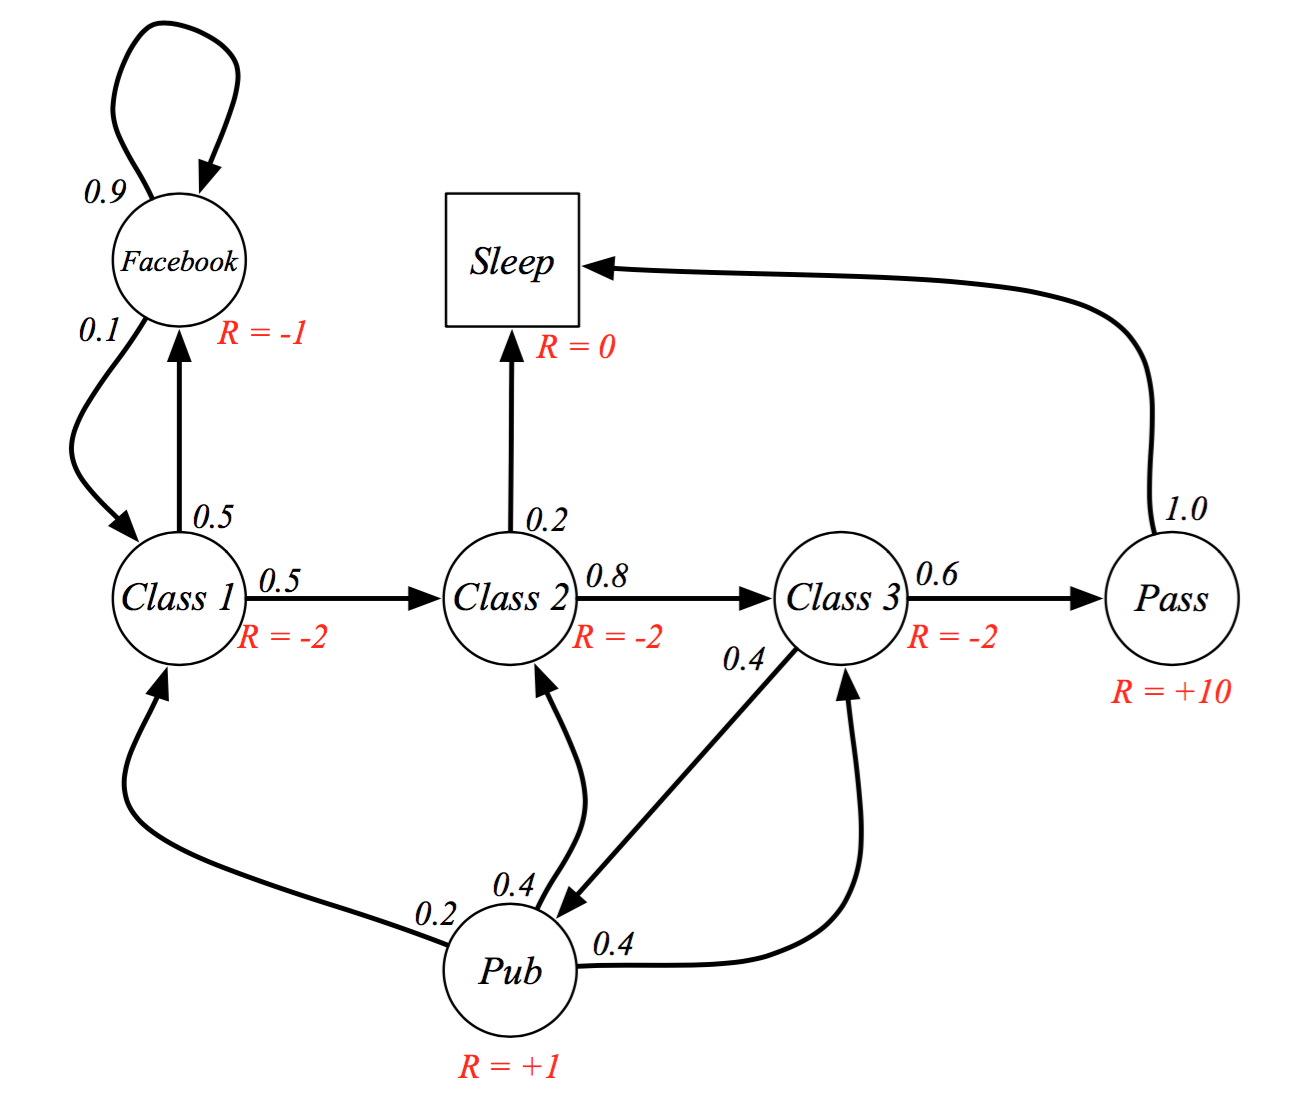
\includegraphics[width=9cm]{reward.png}
    \end{figure}
  }
\end{frame}

\begin{frame}
  \frametitle{Learning Methods}
  \begin{block}{Goal}
    Discover an optimal policy that maximizes:
    $$J=E\{\Sigma_{h=0}^HR_h\}$$
    Where $H$ is the steps the algorithm takes
  \end{block}

  \begin{exampleblock}{Expanding}
    Expanding the above with reward settings:
    $$\max_{\pi}J(\pi) = \Sigma_{s,a}\mu^{\pi}(s)\pi(s, a)R(s, a)$$
    $$s.t. \mu^{\pi} = \Sigma_{s,a}\mu^{\pi}(s)\pi(s, a)T(s,a,s'),
    \forall s'\in S,$$
    $$1 = \Sigma_{s,a}\mu^{\pi}(s)\pi(s, a)$$
    $$\pi(s, a)\le 0, \forall s\in S, a\in A$$
    
    Where $\mu$ is the distribution of states.
  \end{exampleblock}
\end{frame}

\begin{frame}
  \frametitle{Simulation}
  \begin{block}{Environment}
    \begin{itemize}
    \item Unity
    \item UR10 Avatar
    \item Simulated Data
    \item Ikpy
    \end{itemize}
  \end{block}
\end{frame}

%%% Local Variables:
%%% mode: latex
%%% TeX-master: "demo"
%%% End:



\begin{frame}[standout]
  Questions?
\end{frame}

\appendix

\begin{frame}[fragile]{Backup slides}
  Sometimes, it is useful to add slides at the end of your presentation to
  refer to during audience questions.

  The best way to do this is to include the \verb|appendixnumberbeamer|
  package in your preamble and call \verb|\appendix| before your backup slides.

  \themename will automatically turn off slide numbering and progress bars for
  slides in the appendix.
\end{frame}

\begin{frame}[allowframebreaks]{References}

  \bibliography{demo}
  \bibliographystyle{abbrv}

\end{frame}

\end{document}

%%% Local Variables:
%%% mode: latex
%%% TeX-master: t
%%% End:
